\documentclass[12pt]{article}

% Idioma y acentos
\usepackage[spanish]{babel}
\usepackage[utf8]{inputenc}
\usepackage[T1]{fontenc}
\usepackage{float}

% Márgenes y tipografía
\usepackage[a4paper, margin=2.5cm]{geometry}
\usepackage{lmodern}
\usepackage{setspace}
\onehalfspacing

% Imágenes y colores
\usepackage{graphicx}
\usepackage{xcolor}

% Para centrar verticalmente en la carátula
\usepackage{titling}

\begin{document}
\begin{titlepage}
    \centering

    
\includegraphics[width=3cm]{imagen/logo-una.png}\par\vspace{1cm} %SUBIMOS LOGO 


    {\large \textbf{Universidad Nacional de Asuncion}}\par
    {\large Facultad Politecnica}\par
    \vspace{2cm}

    % TÍTULO
    {\Huge \textbf{Desarrollo de una Estrategia de Fusión de
                Datos FTIR y Raman para la
                Caracterización Avanzada de Muestras
                mediante Análisis Multivariado}}\par
    \vspace{0.5cm}
    {\Large Guia de Usuario - EspectroApp}\par
    \vspace{2cm}


    \large \textbf{Diego Hyung Won Seo Gonzalez}\par
    \large \textbf{Ricardo Jesus Leguizamon Acosta}\par
    \vspace{0.8cm}

    % TUTOR(ES) / CÁTEDRA (opcional)
    {\large \textbf{Tutor:} Julio Mello}\par
    \vspace{2cm}

    % LUGAR Y FECHA
    {\large San Lorenzo, Paraguay}\par
    {\large \today}\par
\end{titlepage}

\section{Introducción}
EspectroApp es un software desarrollado en Python con interfaz gráfica basada en PySide6 (Qt), diseñado para la visualización, preprocesamiento y análisis avanzado de datos espectroscópicos (principalmente Raman y FTIR).
Su objetivo es facilitar a investigadores y estudiantes el tratamiento de grandes conjuntos de espectros mediante un entorno interactivo que integra:
\begin{itemize}
    \item Carga y gestión de datos en formatos .csv y .txt.
    \item Transformaciones espectrales: normalización, suavizado, corrección de línea base, etc.
    \item Reducción de dimensionalidad mediante PCA, t-SNE y HCA.
    \item Modelos de fusión de datos (Low-Level, Mid-Level) para integrar información de diferentes técnicas espectroscópicas.
    \item Visualización interactiva con gráficos dinámicos usando PyQtGraph, Matplotlib y Plotly.
\end{itemize}
En resumen, EspectroApp combina procesamiento matemático, machine learning básico y herramientas gráficas interactivas para ofrecer una plataforma ágil y adaptable en el análisis de espectros


\newpage
    \section{Guía de Instalación – EspectroApp}
    
    \subsection*{Requisitos previos}
    
    \begin{enumerate}
        \item \textbf{Hardware mínimo recomendado:}
        \begin{itemize}
            \item \textbf{Procesador:} Intel i3 / AMD Ryzen 3 o superior
            \item \textbf{Memoria RAM:} mínimo 4 GB
            \item \textbf{Espacio en disco:} 1 GB libre
        \end{itemize}
    
        \item \textbf{Sistema operativo compatible:}
        \begin{itemize}
            \item Windows 10 / 11 (64 bits)
            \item Linux (Ubuntu 20.04+, Debian 12+, Fedora 38+, etc.)
        \end{itemize}
    
        \item \textbf{Instalación en Windows:}
        \begin{itemize}
            \item Descargue el archivo ejecutable EspectroApp.exe desde la carpeta de distribución
            \item Copie el archivo a una carpeta de su preferencia (por ejemplo, \verb|C:\EspectroApp|).
            \item Haga doble clic en EspectroApp.exe.
            \item Si aparece el mensaje de seguridad de Windows SmartScreen:
                \begin{enumerate}
                    \item Haga clic en Más información.
                    \item Seleccione Ejecutar de todas formas.
                \end{enumerate}
        \end{itemize}
    
    
        \item \textbf{Instalación en Linux:}
        \begin{itemize}
            \item Descargue el archivo ejecutable EspectroApp.exe desde la carpeta de distribución
            \item Copie el archivo a una carpeta de su preferencia con los siguientes comandos.
                \begin{enumerate}
                    \item mkdir -p ~/EspectroApp
                    \item cd EspectroApp ~/EspectroApp/
                    \item cd ~/EspectroApp
                \end{enumerate}
            \item Dé permisos de ejecución al binario (solo la primera vez):
                \begin{enumerate}
                    \item chmod +x EspectroApp
                \end{enumerate}
            \item Ejecute el programa:
                \begin{enumerate}
                    \item ./EspectroApp
                \end{enumerate}
        \end{itemize}
    \end{enumerate}
        
\newpage   
    \subsection*{Entorno y dependencias}
    
    El software \textbf{EspectroApp} fue desarrollado y probado con el siguiente entorno de Python y librerías:
    
    \begin{table}[H]
    \centering
    \renewcommand{\arraystretch}{1.2}
    \begin{tabular}{|l|c|p{7cm}|}
    \hline
    \textbf{Biblioteca / Entorno} & \textbf{Versión} & \textbf{Uso en EspectroApp} \\
    \hline
    Python          & 3.12.x   & Intérprete principal del software \\
    PySide6         & 6.9.2    & Interfaz gráfica de usuario (Qt) \\
    shiboken6       & 6.9.2    & Soporte interno para PySide6 \\
    numpy           & 2.3.2    & Cálculos numéricos y manejo de matrices \\
    pandas          & 2.3.2    & Manipulación de datos espectrales (CSV/TXT) \\
    matplotlib      & 3.10.6   & Gráficos estáticos de espectros \\
    pyqtgraph       & 0.13.3   & Visualización rápida e interactiva de espectros \\
    plotly          & 6.3.0    & Gráficos interactivos (PCA, t-SNE, etc.) \\
    scikit-learn    & 1.7.1    & Métodos de reducción de datos (PCA, t-SNE, clustering) \\
    scipy           & 1.16.1   & Procesamiento matemático y científico \\
    seaborn         & 0.13.2   & Mapas de calor y visualización estadística \\
    joblib          & 1.5.2    & Serialización y paralelización de modelos \\
    threadpoolctl   & 3.6.0    & Control de hilos en cálculos intensivos \\
    altgraph        & 0.17.4   & Soporte interno de PyInstaller \\
    pyinstaller     & 6.15.0   & Creación de ejecutables (Windows/Linux) \\
    pillow          & 11.3.0   & Manejo de imágenes (logos, iconos) \\
    python-dateutil & 2.9.0    & Manejo de fechas en datasets \\
    pytz / tzdata   & 2025.2   & Soporte de zonas horarias \\
    setuptools      & 80.9.0   & Construcción e instalación de paquetes \\
    \hline
    \end{tabular}
    \end{table}

\newpage
    \section{Menu Principal - Carga y Visualizacion}
    % poner aca la imagen de los primeros 3 botones
    \subsection{Cargar Archivo}
    \textbf{Objetivo:} Seleccionar los archivos con los datos espectrales que se desean visualizar.
    \textbf{Pasos rápidos}
    \begin{enumerate}
      \item Dar click en el boton \textbf {Cargar Archivo}
      \item Moverse hasta la carpeta en donde se encuentra el archivo con los datos
    \end{enumerate}
    
    \textbf{Resultado:} Guarda lo/s dato/s dentro de un diccionario global en donde se almacenaran todos los archivos seleccionados.
    
    \textbf{Errores comunes \& soluciones}
    \begin{itemize}
      \item Tratar de cargar una carpeta en vez de un archivo
      \item Formato del archivo con extension diferente al .csv
    \end{itemize}
    
    \begin{figure}[H]\centering
      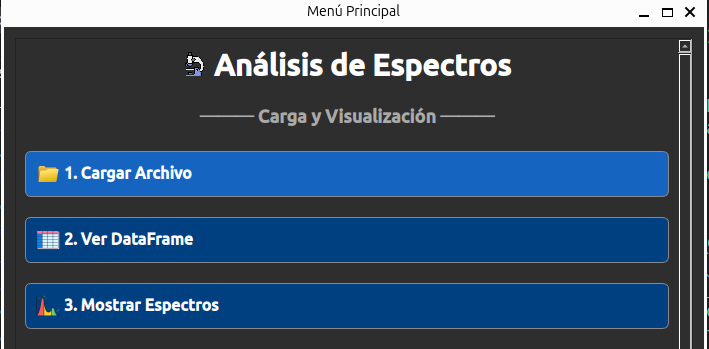
\includegraphics[width=.85\linewidth]{imagen/cargararchivo.png}
      \caption{Botón Cargar Archivo}
      \small Fuente: Producida por el autor
    \end{figure}
    

    \subsection{Ver DataFrame}
    \textbf{Objetivo:} Seleccionar los archivos con los datos espectrales que se desean visualizar.
    \textbf{Cuándo usarlo:} Esta opcion se utilizara cuando queramos ver los dataframe cargados o los resultados de algun tipo de procesamiento que hallamos aplicado.
 
    \textbf{Pasos rápidos}
    \begin{enumerate}
      \item Dar click en \textbf{Ver DataFrame}
      \item Aparecera una ventana donde se podran visualizar todos los archivos cargados anteriormente en \textbf{Cargar Archivo} con algunas informaciones basicas como cantidad de columna, filas o numeros null
      \item A su derecha se podran observar dos botones uno para ver su respectivo archivo y la otra para borrarla
    \end{enumerate}

    % (opcional) captura de pantalla
    \begin{figure}[H]\centering
      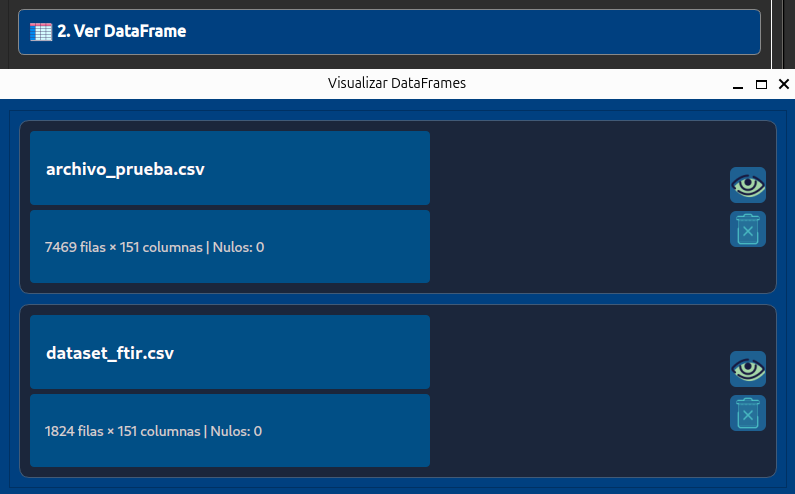
\includegraphics[width=.85\linewidth]{imagen/verdataframe.png}
      \caption{Botón Ver Dataframe}
      \small Fuente: Producida por el autor
    \end{figure}


    \subsection{Mostrar Espectros}
    \textbf{Objetivo:} Visualizar gráficamente los espectros cargados para inspección, análisis comparativo o exportación.
    \textbf{Cuándo usarlo:} Cuando el usuario necesite visualizar los espectros cargados para verificar ruido, detectar valores atípicos o centrarse en una región específica.
    \textbf{Pasos:}
    \begin{enumerate}
      \item Dar clic en el botón \textbf{Mostrar Espectros}.
      \item Seleccionar el modo de visualización: completo, por muestra o acotado.
      \item Ajustar parámetros (ejemplo: rango de interés en modo acotado o muestra en especifico).
      \item Confirmar para visualizar el gráfico o descargarlo.
    \end{enumerate}

    % (opcional) captura de pantalla
    \begin{figure}[H]\centering
      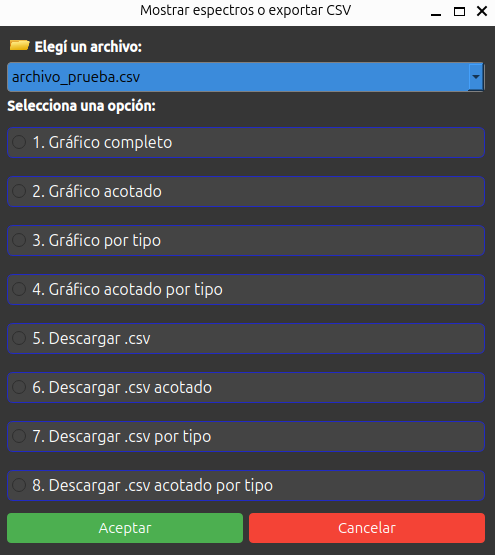
\includegraphics[width=.85\linewidth]{imagen/mostrararchivo.png}
      \caption{Botón Mostrar Espectro}
      \small Fuente: Producida por el autor
    \end{figure}


    \section{Menu Principal - Procesamiento}
    \subsection{Procesar Datos}
    \textbf{Objetivo:} Aplicar transformaciones y preprocesamiento a los espectros cargados para mejorar la calidad de los datos antes de la reducción de dimensionalidad o la fusión.
    \textbf{Cuándo usarlo:} Cuando los espectros presentan ruido, desplazamientos de línea base o requieren normalización para ser comparables entre sí.
    \textbf{Pasos:}
    \begin{enumerate}
      \item Dar clic en el botón \textbf{Procesar Datos}.
      \item Seleccionar el \textbf{DataFrame} a transformar.
      \item Marcar las casillas con el metodo de procesamiento que se desea realizar.
      \item \textbf{Normalización Media:} estandariza los datos como muestra la figura 4
         % (opcional) captura de pantalla
        \begin{figure}[H]\centering
          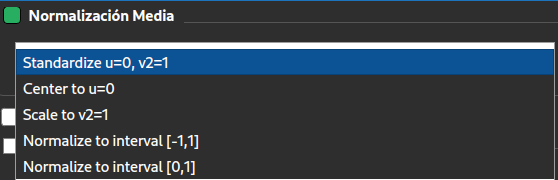
\includegraphics[width=.85\linewidth]{imagen/normalizacionmedia.png}
          \caption{CheckBox Normalizacion por la media}
          \small Fuente: Producida por el autor
        \end{figure}
      \item \textbf{Normalizar por área:} ajusta los espectros para que tengan igual área total.
       \item \textbf{Suavizado Savitzky-Golay:} solicita definir \emph{ventana} (número de puntos, ej. 5) y \emph{orden} del polinomio (ej. 2).
      \item \textbf{Suavizado Filtro Gaussiano:} solicita definir el valor de \emph{sigma}.
      \item \textbf{Suavizado Media Móvil:} solicita definir el tamaño de \emph{ventana}.
      \item \textbf{Derivadas:} calcular primera o segunda derivada del espectro.
      \item \textbf{Corrección de línea base:} opción lineal o método de Shirley.
      \item Presionar \textbf{Aceptar} para procesar el dataframe y asignar un nuevo nombre al dataframe procesado.
    \end{enumerate}

    \begin{figure}[H]\centering
      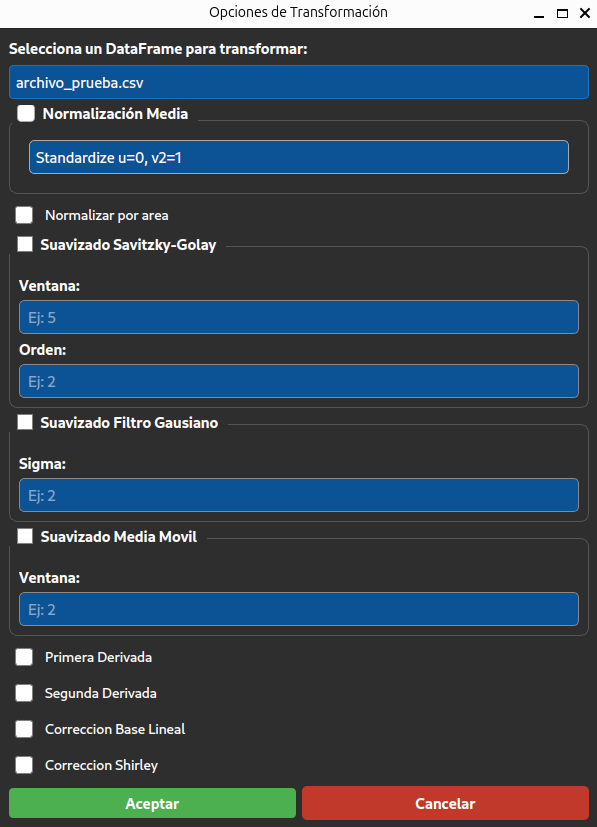
\includegraphics[width=.65\linewidth]{imagen/procesardatos.png}
      \caption{Botón Procesar Datos}
      \small Fuente: Producida por el autor
    \end{figure}

  
    \subsection{Reduccion de Dimensionalidad}
    \textbf{Objetivo:} Representar espectros de alta dimensionalidad en un espacio reducido (2D o 3D), facilitando la visualización de patrones, la clasificación y la detección de agrupamientos.\\
    \textbf{Cuándo usarlo:} Cuando se necesita explorar relaciones entre muestras, identificar similitudes, diferencias y simplificar el análisis visual de grandes volúmenes de datos espectrales.
    \textbf{Pasos rápidos}
    \begin{enumerate}
      \item Dar clic en el botón \textbf{Reducción de Dimensionalidad}.
      \item Seleccionar el \textbf{DataFrame} que contiene los datos.
      \item Elegir la técnica de reducción:
            \begin{itemize}
                \item  \textbf{PCA (Análisis de Componentes Principales):} reduce la dimensionalidad maximizando la varianza explicada.
                \item  \textbf{t-SNE:} proyecta datos en 2D o 3D conservando relaciones de proximidad entre muestras.
                \item \textbf{t-SNE(PCA(X)):} aplica primero PCA y luego t-SNE, útil para conjuntos grandes de datos.
            \end{itemize}
    \item Definir parámetros:
    \begin{itemize}
      \item \textbf{PCA:} Ingresamos la cantidad de componentes principales n>=2.
      \item \textbf{t-SNE:} Ingresamos la cantidad de componentes principales n = 2 o n =3
      \item \textbf{Intervalo de Confianza:} define el nivel de confianza para elipses en las gráficas (ej. 90\%).
    \end{itemize}
  \item Seleccionar las salidas deseadas:
    \begin{itemize}
      \item \textbf{Gráfico 2D:} proyección en dos dimensiones, Ingresar componentes a graficar en eje X y eje Y respectivamente.
      \item \textbf{Gráfico 3D:} proyección tridimensional interactiva. Ingresar componentes a graficar en eje X, eje Y y eje Z.
      \item \textbf{Gráfico Loading (PCA):} muestra la contribución de cada variable/espectro en los componentes.
      \item \textbf{Generar Informe:} crea un reporte con los resultados de los parámetros ingresados.
    \end{itemize}
      \item Presionar \textbf{Aceptar} para ejecutar o \textbf{Cancelar} para salir sin cambios.\\
    \textbf{Salida:} Gráficos en dos o tres dimensiones y informe automatizado con los resultados.
    
    \textbf{Errores comunes y soluciones:}
    \begin{itemize}
      \item \textit{El gráfico aparece vacío:} verificar que se haya cargado un DataFrame válido y verificar que se haya ingresado los componentes como eje 
      \item \textit{Resultados poco claros en t-SNE:} ajustar parámetros como \emph{perplexity} e incrementar iteraciones.
      \item \textit{Elipse de confianza no aparece:} confirmar que el intervalo esté en valores aceptados (90, 95 o 99).
      \item \textit{Verificar las versiones instaladas de las librerias de Python.}
    \end{itemize}
    \end{enumerate}

    % (opcional) captura de pantalla
    \begin{figure}[H]\centering
      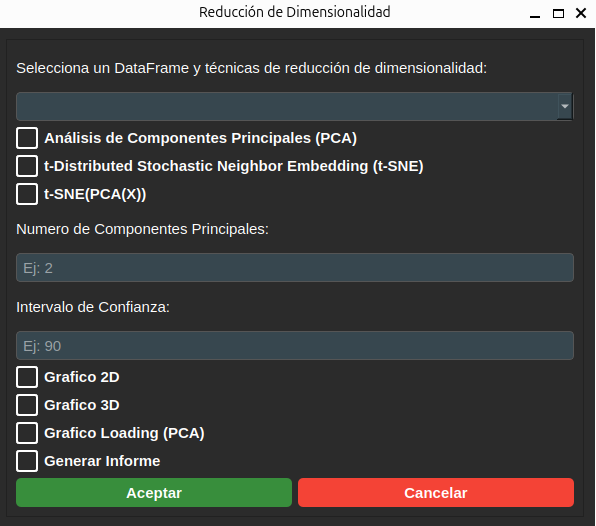
\includegraphics[width=.85\linewidth]{imagen/reducciondimensionalidad.png}
      \caption{Botón Reduccion Dimensionalidad}
      \small Fuente: Producida por el autor
    \end{figure}


    \subsection{Analisis Jerarquico(HCA)}
    \textbf{Objetivo:} Agrupar muestras en función de sus espectros y representarlas mediante un dendrograma jerárquico.
    \textbf{Cuándo usarlo:} Cuando se necesita identificar grupos naturales de muestras o explorar similitudes

    \textbf{Pasos:}
    \begin{enumerate}
      \item Dar clic en el botón \textbf{Análisis Jerárquico}.
      \item Seleccionar el DataFrame.
      \item Marcar la casilla con el método a utilizar para realizar el cálculo de sus distancias.
      \item Marcar la casilla con el método de cluster a utilizar. 
            El método Ward solo puede ser utilizado junto a la distancia Euclidiana o Manhattan.
    \end{enumerate}
    
    \begin{figure}[H]\centering
      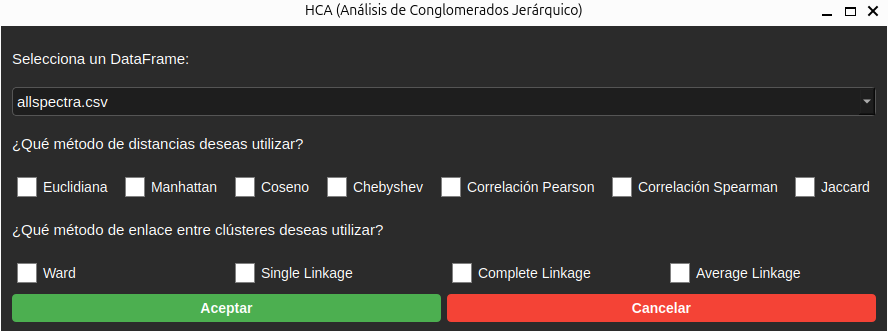
\includegraphics[width=.95\linewidth]{imagen/hca.png}
      \caption{Botón Análisis Jerárquico}
      \small Fuente: Producida por el autor
    \end{figure}
    
    \textbf{Ejemplo de salida:}  
    Los números que se observan en el eje X son las muestras del archivo. Para saber cuáles muestras representa cada número, el software genera un archivo llamado \textbf{grupos\_hca.txt}.
    
    \begin{figure}[H]\centering
      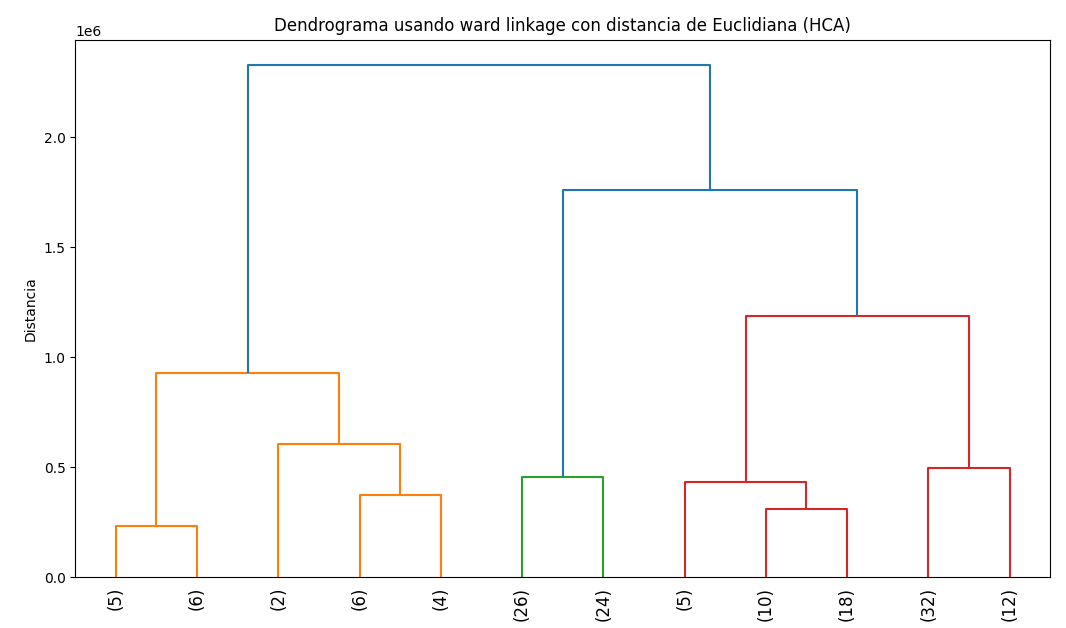
\includegraphics[width=.95\linewidth]{imagen/hcaejemplo.png}
      \caption{Ejemplo Analisis Jerarquico}
      \small Fuente: Producida por el autor
    \end{figure}

\newpage
\section{Menu Principal - Fusion}
\textbf{Objetivo:} Combinar dos o más conjuntos de espectros por ejemplo (Raman y FTIR) para obtener una representación conjunta que mejore la separación, visualización y análisis de las muestras.\\
    \textbf{Cuándo usarlo:} Cuando tengas varias técnicas para las \textit{mismas} muestras y quieras integrar su información antes de analizar (PCA, t-SNE, HCA). \\
    \textbf{Requisitos:}
   \begin{itemize}
   \item Haber cargado previamente los archivos a fusionar.
   \item Las muestras deben estar ordenados de la misma forma en todos los archivos con los mismo nombres
    \end{itemize}
    \textbf{Flujo de uso}
    \begin{enumerate}
      \item Dar clic en \textbf{Data Fusion}. Se abre una ventana con la lista de archivos cargados. 
            Selecciona los que deseas fusionar.
      \item Se abre una segunda ventana con las informaciones de los archivos:
            el sistema verifica si existe intersección entre sus ejes x.
      \item Según el resultado, elige el \textbf{rango de trabajo}:
            \begin{itemize}
              \item \textbf{Rango completo:} interpola cada señal en todo su rango original.
              \item \textbf{Solo intersección:} interpola únicamente la parte comun común.
            \end{itemize}
      \item Define la \textbf{interpolación} y el \textbf{paso}:
            \begin{itemize}
              \item \textit{Tipo de interpolación:} lineal, spline/cúbica, polinómica, etc.
              \item \textit{Paso:} para formar el nuevo eje x puede ser ingresando un numero(paso) directamente, paso igual al promedio o definir un numero fijo de puntos.
              \item  \textit{No hay interseccion:} para ese caso la unica opcion posible de elegir un paso seria ingresando directamente un numero fijo de puntos.
            \end{itemize}
      \item Elige el \textbf{nivel de fusión}:
            \begin{itemize}
              \item \textbf{Low-Level Fusion:} marca \textit{tipo de interpolación} y \textit{paso}. 
                    Concatena las señales ya en el mismo eje.
              \item \textbf{Mid-Level Fusion:} además de \textit{tipo de interpolación} y \textit{paso}, 
                    indica número de Componentes Principales (PCA) por técnica y el 
                    intervalo de confianza para las gráficas.
            \end{itemize}
      \item Ejecuta la opción deseada:
            \begin{itemize}
              \item Botón \textbf{Low Fusion} → genera y grafica la fusión de bajo nivel.
              \item Botón \textbf{Mid Level} → genera y grafica la fusión de nivel medio.
            \end{itemize}
    \end{enumerate}
    
    \textbf{Salida:}
    \begin{itemize}
      \item Matriz fusionada (low: señales concatenadas; mid: \textit Componentes concatenadas por PCA).
      \item Gráficos 2D/3D y si corresponde, elipses de confianza.
    \end{itemize}
    
    \textbf{Errores comunes y soluciones}
    \begin{itemize}
      \item \textit{Diferente número de muestras:} verifica que los archivos correspondan a las mismas muestras y orden.
      \item \textit{Gráfico vacío o distorsiones:} reduce el paso o cambia el metodo de interpolación.
    \end{itemize}
    
\end{document}



























